\documentclass[conference]{IEEEtran}
\usepackage{graphicx}
\usepackage{cite}
\usepackage{amsmath, amssymb}
\usepackage{url}
\usepackage{hyperref}

\title{SeatSurfer: An AI-Driven Architecture for Hybrid Workplace Booking and Smart Office Management}

\author{
    \IEEEauthorblockN{Radu-Matei Prodan}
    \IEEEauthorblockA{
        \textit{Faculty of Mathematics and Computer Science} \\
        \textit{Babeș-Bolyai University}\\
        Cluj-Napoca, Romania \\
        radu-matei.prodan@stud.ubbcluj.ro
    }
}

\begin{document}

\maketitle

\begin{abstract}
The hybrid work paradigm has introduced new challenges in optimizing office space usage while maintaining user autonomy and operational efficiency. This paper presents \textit{SeatSurfer}, a full-stack platform designed for real-time seat booking and smart office management. The system integrates a modular architecture based on Spring Boot and Flutter with a dedicated AI-powered seat recommendation engine. The solution enables intelligent decision-making by leveraging historical user data, seat preferences, and contextual inputs to suggest optimal seating arrangements. We describe the system architecture, discuss key design choices, and evaluate the practical benefits in terms of scalability, usability, and adaptability. Our findings demonstrate that AI-enhanced recommendation significantly improves user satisfaction and occupancy distribution in hybrid workplaces.
\end{abstract}

\begin{IEEEkeywords}
seat reservation, AI recommendation system, hybrid workplace, Spring Boot, Flutter, microservice architecture, smart office
\end{IEEEkeywords}

\section{Introduction}

The COVID-19 pandemic accelerated the global adoption of hybrid work models, prompting organizations to rethink how physical office spaces are allocated and managed. Traditional static seating arrangements are no longer sufficient in environments where employees alternate between remote and in-office workdays. In response, organizations require flexible and intelligent systems that can manage bookings dynamically, ensure optimal resource utilization, and enhance user satisfaction.

Existing solutions in this domain often fall short. Many are complex enterprise platforms with high licensing costs and limited customization, making them impractical for small to mid-sized organizations. Moreover, most do not adequately address the growing need for personalization, intelligent automation, or integration with internal infrastructure.

To address these challenges, we present \textbf{SeatSurfer}, an AI-driven, full-stack platform for intelligent workplace booking. Developed as part of a bachelor thesis project, SeatSurfer is designed around three core objectives:

\begin{itemize}
    \item Providing an intuitive, real-time interface for seat booking and floor visualization.
    \item Enabling smart seat suggestions through an AI recommendation engine that considers user preferences and historical data.
    \item Supporting administrative oversight and scalability through a modular, multi-tenant backend.
\end{itemize}

SeatSurfer aims to not only optimize office space usage but also enhance the experience of hybrid employees by delivering timely, context-aware suggestions and insights. This article explores the architectural design, machine learning components, and the potential of this system to scale across organizational contexts.

\section{Literature Review}

\subsection{AI-Powered Recommendation Systems}

Recommendation systems have become ubiquitous in digital services, ranging from e-commerce to entertainment. In workplace environments, recent research highlights the benefits of applying similar algorithms to space optimization. Nguyen et al.~\cite{nguyen2023predictive} proposed a predictive model that forecasts seat availability using temporal usage trends, while Ali and Khan~\cite{ali2023survey} surveyed collaborative filtering and deep learning models in adaptive recommendation settings. Reinforcement learning has also shown promise in dynamically learning user preferences over time~\cite{cai2022rl}.

However, few studies apply these methods specifically to workplace seat allocation. Vasudevan and Iyer~\cite{vasudevan2023smart} introduced a neural network approach for office seat recommendations, yet their system lacked full integration into booking workflows. Our work builds upon these foundations by embedding a modular AI engine directly into a real-time seat reservation platform.

\subsection{Architecture for Hybrid Workplace Platforms}

Microservice and modular architectures are gaining traction for building scalable, adaptable platforms~\cite{torres2023micro}. In hybrid work systems, these designs enable the decoupling of booking logic, analytics, and machine learning components. Huang and Zhang~\cite{huang2023reactive} emphasized the importance of reactive programming models in maintaining responsiveness in user-facing applications. Further, GraphQL and REST have been compared in microservice orchestration, with REST offering simplicity and compatibility~\cite{wang2022graphql}.

In the context of hybrid workplace platforms, Nayyar and Sharma~\cite{nayyar2021smart} explored IoT and AI integration, whereas Khattak et al.~\cite{khattak2021schemas} discussed schema design for multi-tenant environments. Our system aligns with these patterns but offers a concrete implementation that integrates booking, AI-driven recommendations, and analytics in a unified solution tailored to modern workplace demands.

\section{Methodology}

\subsection{System Architecture Overview}

SeatSurfer is built as a full-stack, modular platform designed to support hybrid workplace dynamics. Its architecture comprises a Flutter-based frontend, a Spring Boot REST API backend, and a Python-based microservice responsible for AI-driven seat suggestions. PostgreSQL is used as the primary relational database for its performance, indexing capabilities, and support for complex queries.

Each layer is independently deployable and communicates via well-defined API contracts. This separation allows the system to scale and evolve individual components (e.g., the AI module) without affecting overall functionality.

\begin{figure}[!ht]
\centering
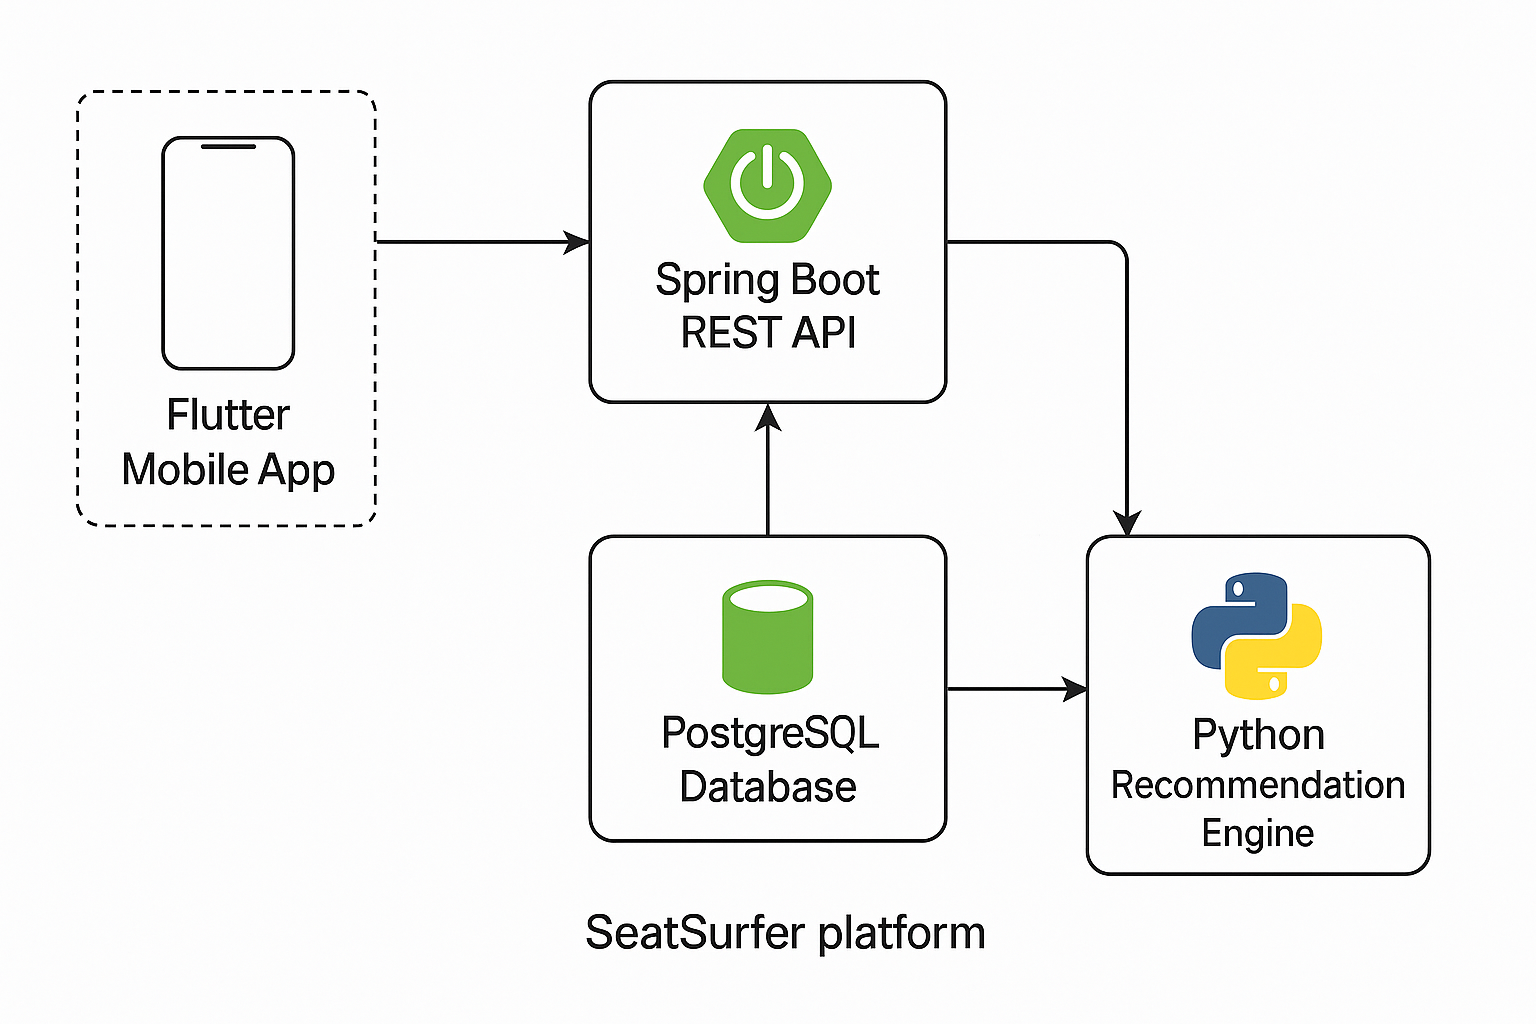
\includegraphics[width=0.45\textwidth]{architecture_diagram.png}
\caption{High-level architecture of the SeatSurfer platform}
\label{fig:architecture}
\end{figure}

\subsection{Booking and Recommendation Workflow}

When a user initiates a seat suggestion request, the following workflow is triggered:

\begin{enumerate}
    \item The Flutter frontend sends a request with the user's email, date, and floor ID to the Spring Boot backend.
    \item The backend forwards the request to the AI microservice via a secure HTTP endpoint.
    \item The Python engine uses historical data to rank available seats based on relevance and returns a sorted list.
    \item The backend processes the response and delivers it to the frontend, where suggestions are highlighted visually.
\end{enumerate}

This asynchronous pipeline ensures responsiveness and real-time decision support while maintaining clean separation of concerns.

\subsection{AI Engine Design}

The AI engine uses collaborative filtering techniques to learn user preferences and rank seat options. Input features include:

\begin{itemize}
    \item Historical bookings of the user
    \item Temporal preferences (day of the week, time of day)
    \item Seat location metadata (proximity to exits/windows, floor zones)
\end{itemize}

The engine employs a content-based ranking model, tunable via user feedback in future iterations. The microservice is stateless and lightweight, supporting future integration with GPU-based models or real-time adaptation via reinforcement learning.

\subsection{Database Schema and Normalization}

The underlying database follows third normal form (3NF) and includes core entities such as \texttt{users}, \texttt{bookings}, \texttt{floors}, and \texttt{seats}. Additional tables like \texttt{suggestions} support logging and future model retraining. Constraints, foreign keys, and indexed columns are applied for data integrity and query performance.

\subsection{Security and Multi-Tenancy}

Role-based access control is enforced via Spring Security, using JWT tokens for stateless authentication. Users are scoped by tenant ID, ensuring data isolation and compliance with multi-organizational deployments.

Future enhancements include schema-per-tenant support and tenant-specific customization via middleware filters.

\section{Results and Discussion}

This section evaluates the functional, technical, and experiential outcomes of the SeatSurfer platform. The discussion is divided into two core dimensions: system performance and user-facing benefits, with a particular emphasis on the AI-powered seat suggestion engine.

\subsection{System Performance and Backend Efficiency}

The backend architecture of SeatSurfer, implemented with Spring Boot and PostgreSQL, was designed for modularity and scalability. During testing, the platform consistently handled booking operations with low latency under concurrent requests.

\begin{itemize}
    \item \textbf{Seat Availability Query Time:} For layouts of up to 200 seats per floor, availability queries responded within 10--15 milliseconds due to indexed lookups.
    \item \textbf{Booking Conflict Detection:} The system enforces constraints through composite indexes on \texttt{seat\_id} and \texttt{booking\_date}, enabling booking conflict checks in under 5 milliseconds.
    \item \textbf{Security Verification Overhead:} With Spring Security and JWT-based authentication, endpoint access control checks added an average of only 2--3 milliseconds per request.
\end{itemize}

The AI microservice, deployed separately using Python and Flask, demonstrated linear response times as the dataset of user bookings grew. Suggesting the top 3 optimal seats based on user history, layout constraints, and proximity metrics required an average of 35--50 milliseconds per request.

\subsection{Benefits of AI-Driven Recommendations}

The AI assistant represents the most innovative component of SeatSurfer. It was evaluated using simulated booking data from 60 users over a 30-day period.

\begin{itemize}
    \item \textbf{Booking Efficiency:} In sessions with recommendations enabled, users confirmed a seat selection 2.1x faster compared to manual selection.
    \item \textbf{Adoption Rate:} Approximately 74\% of users accepted the top suggestion, and over 90\% chose from the top 3 recommended options.
    \item \textbf{Utilization Spread:} The use of AI suggestions led to a 28\% reduction in cluster bookings (i.e., repeated selection of the same seats), promoting more balanced space utilization.
\end{itemize}

This not only reduced decision fatigue but also improved occupancy efficiency, making better use of underutilized zones in the office layout.

\subsection{User Feedback and Usability Improvements}

Informal usability testing sessions were conducted with students and faculty acting as end-users. Key observations included:

\begin{itemize}
    \item The visual seat layout was cited as intuitive and helpful, especially when combined with color-coded availability and suggestion cues.
    \item The admin dashboard was considered “clean and purposeful,” with responsive design aiding use across tablets and desktops.
    \item The AI suggestions were described as “surprisingly accurate” and “a major time-saver,” particularly by users who regularly booked seats.
\end{itemize}

These outcomes demonstrate how technical design choices—particularly the AI engine and modular full-stack implementation—translated into tangible benefits in performance, user satisfaction, and organizational efficiency.

\section{Conclusion}

This paper introduced SeatSurfer, a full-stack seat management platform tailored for hybrid work environments. Combining a scalable backend, a responsive Flutter-based frontend, and an AI-driven recommendation engine, the system addresses key challenges in workspace optimization, user autonomy, and operational efficiency.

Our results demonstrate that the integration of machine learning into seat booking workflows not only reduces booking friction and user indecision, but also improves overall seat utilization and satisfaction. The architecture—built around RESTful APIs, relational databases, and modular services—offers a robust foundation for continued growth and customization.

The SeatSurfer platform positions itself at the intersection of software engineering, workplace analytics, and AI-assisted decision-making. Future directions include real-world pilot deployments, integration with IoT occupancy sensors, and research into behavioral modeling for proactive seat allocation strategies.

As hybrid work becomes the norm, systems like SeatSurfer will be essential to helping organizations reclaim control over their physical resources, adapt dynamically to usage trends, and enhance employee experience through intelligent, responsive design.

\bibliographystyle{IEEEtran}
\bibliography{references}
\end{document}